\chapter{Mathematics and Computers: How Far Can Algorithms Go?}

\section{After Ten Million Successes}

Start with a game. Write any positive integer and repeatedly apply this rule: if even, divide by $2$; if odd, multiply by $3$ and add $1$. Starting with $6$ gives

\[6 \to 3 \to 10 \to 5 \to 16 \to 8 \to 4 \to 2 \to 1.\]

After reaching $1$, the number $1$ becomes $4$, then $4$ becomes $2$, and $2$ returns to $1$, entering the cycle $4 \to 2 \to 1$. We stop there.

The rule could scarcely be simpler, yet its question has defeated the world. Mathematicians conjecture that \textbf{every} positive starting integer reaches $4 \to 2 \to 1$ after finitely many steps. This is the famous "$3n+1$ conjecture", also called the Collatz, Kakutani, or hailstone conjecture: numbers often rise and fall before descending, like hail tumbling in a cloud.

The conjecture remains neither proved nor disproved. But people tried something blunt: let computers test it. An ordinary laptop checks millions of numbers per second; specialist teams using large computers have verified every integer from $1$ to about $2^{68}$, approximately thirty quadrillion. \textbf{Every number} eventually reached $4 \to 2 \to 1$, with no exceptions.

Thirty quadrillion successes, no exceptions. Has the conjecture now been proved?

Many instinctively say yes: surely that many tests settle it. Others hesitate: could a counterexample hide much farther out? Starting from that hesitation, we explore mathematics' close yet subtle relationship with computers: what can machines do for mathematics, and what can they never do?

\section{Why Is So Much Verification Still Not Proof?}

Before taking sides, consider historical stories showing how unreliable repeated success can be.

\subsection{A Formula That Fooled Us Forty Times}

Consider $n^2 - n + 41$. At $n=1$ it gives $41$, prime; $n=2$ gives $43$, prime; $n=3$ gives $47$, again prime. Continue through $n=4,5,6,\dots$ and obtain $43,47,53,61,71,83,97,\dots$, apparently all prime. In fact, every value from $n=1$ through $n=40$ is prime: forty successes.

A computer might confidently report forty consecutive successes. But at $n=41$,

\[41^2 - 41 + 41 = 41^2 = 41 \times 41,\]

clearly composite. Failure follows immediately after forty successes.

\subsection{A Counterexample Beyond Nine Hundred Million}

If forty seems too few, what about nine hundred million? In 1919, Polya proposed a conjecture about prime distribution. Its details need not concern us; what matters is how overwhelmingly plausible it seemed. Tests found it true for every number up to nine hundred million. At one number per second, checking that many would take over twenty years without sleep or meals.

Yet in 1958 it was proved false, with the smallest counterexample near $906\,150\,257$, just beyond nine hundred million. All the preceding successes had failed to reach the truth's edge. The first exception hid at a place brute force could barely reach.

\subsection{Even Great Mathematicians' Conjectures Can Sink}

In 1769, Euler conjectured, roughly, that at least $n$ numbers raised to the $n$th power must be added to obtain another $n$th power. It stood for nearly two centuries and inspired considerable trust: Euler rarely misjudged such things.

In 1966, two mathematicians used computer search to find a clean counterexample:

\[27^5 + 84^5 + 110^5 + 133^5 = 144^5.\]

Euler's conjecture required at least $5$ fifth powers; this uses only $4$. One equality overturned nearly two centuries of confidence. Notice that a \textbf{computer} helped find it, searching a range impossible by hand. Its role was not prover, but expert fault-finder.

\begin{fanli}
\textbf{Counterexample alert: declaring success after $N$ tests.}

Whether $N$ is a hundred, a million, or thirty quadrillion, the first $N$ successes establish only a \textbf{finite range}. Mathematical conjectures usually concern \textbf{infinitely many} objects, and infinity cannot be exhausted. Finite tests provide \textbf{evidence} and confidence, help \textbf{discover patterns}, and may \textbf{find a counterexample} that disproves the conjecture. They never replace a proof covering every case. Conversely, one counterexample refutes a conjecture, while proving it must address infinitely many possibilities: the difficulties are inherently asymmetric.
\end{fanli}

Return to $3n+1$: thirty quadrillion checks build strong confidence, but Polya's story reminds us that an exception might lurk beyond a hundred septillion. Until proof or counterexample arrives, we must honestly call it a \textbf{conjecture}, not a theorem.

\section{Algorithms: Machines of Thought}

We keep saying to let a computer verify things. What does it actually do? Without eyes or intuition, its fundamental activity is \textbf{executing prewritten instructions step by step}. Such an instruction sequence is an algorithm.

\begin{shuyu}{Algorithm}
\textbf{Intuition}: An instruction manual so precise that someone, or something, with no mathematical understanding can mechanically follow it and obtain a result after finitely many steps.

\textbf{Formal definition}: An algorithm is a finite collection of unambiguous instructions that, for every valid kind of input, terminates after finitely many steps and outputs a definite answer. Finite termination matters: a programme that runs forever does not qualify.

\textbf{Example}: Find the greatest common divisor of two positive integers with the two-thousand-year-old Euclidean algorithm. For $1071$ and $462$, calculate $1071 = 2 \times 462 + 147$, $462 = 3 \times 147 + 21$, and $147 = 7 \times 21 + 0$. Stop at remainder $0$; the answer is $21$. Every step is explicit and termination is guaranteed: a textbook algorithm.
\end{shuyu}

Why care so much about algorithms as a concept? They draw a precise boundary around mechanical calculation. Once defined, we can ask astonishing questions:

\begin{itemize}
\item Can algorithms solve \textbf{every} mathematical problem?
\item If so, could a machine accept any mathematical statement and automatically declare it true or false?
\end{itemize}

The second sounds like the ultimate mathematical dream. Proof would become button-pushing and mathematicians could retire together. Early in the twentieth century, many genuinely held this hope.

\section{Things Algorithms Can Never Do}

The dream shattered in 1936. Considering the nature of computation, the British mathematician Turing asked a simple question: \textbf{can an algorithm decide whether any given programme will halt?}

What is halting? A programme either finishes after finitely many steps, like the Euclidean algorithm, or loops forever, like instructions to start at $1$ and keep adding $1$ without stopping. Halting depends on both code and input. Some loops are obvious; others, such as repeatedly applying $3n+1$ from a large starting number, raise questions nobody knows how to settle.

\begin{dingyi}
\textbf{Halting problem}: Is there an algorithm $H$ that, given any programme $P$ and any input $x$, always answers correctly in finite time whether $P$ halts on $x$?
\end{dingyi}

Turing's answer was earth-shattering: such an algorithm \textbf{does not exist}. Not merely undiscovered, but logically impossible, past, present, and future. This is our central theorem.

\begin{dingli}[Undecidability of the halting problem]
No general algorithm decides whether an arbitrary programme halts on an arbitrary input.
\end{dingli}

\begin{proof}
Argue by contradiction. Suppose algorithm $H$ exists. Given programme text and an input, $H$ always returns ``halts'' or ``does not halt'' after finitely many steps, and is always correct.

Use $H$ as a component to build a strange programme $D$. The only input $D$ accepts is programme text $Q$. The workflow of $D$ is:

\begin{enumerate}
\item Call $H$ and ask whether programme $Q$ halts when given \textbf{its own text} as input.
\item If $H$ says it halts, $D$ deliberately loops forever.
\item If $H$ says it does not halt, $D$ halts immediately.
\end{enumerate}

In short, $D$ is contrary: \textbf{predict halting and I refuse; predict non-halting and I stop}. Constructing $D$ presents no technical obstacle. Given an existing $H$, wrapping it inside $D$ takes only a few lines of code.

Now the crucial move: feed the text of $D$ into $D$ itself. Does $D$ halt when run on $D$?

\begin{itemize}
\item Suppose $D(D)$ halts. Then $H$ must say that $D$ halts on itself. But by the design of $D$, when $H$ says ``halts'', $D$ loops forever, so $D(D)$ does not halt: a contradiction.
\item Suppose $D(D)$ does not halt. Then $H$ must say ``does not halt''. But by the design of $D$, when $H$ says that, $D$ immediately halts, so $D(D)$ halts: another contradiction.
\end{itemize}

Both possibilities contradict themselves. The original assumption must be wrong: $H$ does not exist.
\end{proof}

The cleverness lies in self-reference: ask a judging programme to judge one designed to contradict it. This shares a spirit with the liar paradox, "This sentence is false", and earlier diagonal arguments: \textbf{any system powerful enough to discuss itself risks being bitten by self-reference}.

The implications go beyond programmers lacking a universal loop detector. \textbf{Some mathematical questions have objectively definite answers---a programme either halts or does not---yet no algorithm can systematically find those answers.} Such problems are called uncomputable or undecidable. Many apparently pure mathematical problems are likewise undecidable, including deciding whether an arbitrary system of polynomial equations has integer solutions, Hilbert's tenth problem.

\begin{lianjie}
\textbf{Connection: the halting problem and Godel's incompleteness theorem.}

Earlier we encountered Godel's theorem: every sufficiently strong axiomatic system contains statements true but unprovable within it. This and halting undecidability are two tremors from one earthquake. If a mathematical system were complete enough to decide every statement, we could build a halting decider by submitting the statement that programme $P$ halts. Since halting is undecidable, no complete system can exist. Computation and proof meet at the bottom of the same abyss.
\end{lianjie}

\section{The Chasm Between Fast and Slow: Computational Complexity}

Halting shows that some problems have no algorithm \textbf{in principle}. More practically, among problems that \textbf{do} have algorithms, are all algorithms equally useful?

Clearly not. Compare two:

\textbf{Sequential search}: In a shuffled stack of $n$ bookmarks, find the one holding a maple leaf by checking one at a time. The worst case needs $n$ checks.

\textbf{Binary search}: If bookmarks are sorted by page number, inspect the middle one. If its page is too high, search the left half; if too low, the right. Each check discards half. Searching $n$ bookmarks takes at most $\log_2 n$ checks: $1000$ need only $10$, a million only $20$.

Different algorithms create enormous workload differences for the same question. Computer science classifies problems by the speed of their best algorithms: \textbf{computational complexity}. Its most conspicuous chasm separates two classes:

\begin{itemize}
\item \textbf{Easy-to-solve problems, class P}: An algorithm needs a \textbf{polynomial} number of steps in input size, such as $n$, $n^2$, or $n^3$. Sorting, greatest common divisors, and shortest paths belong here.
\item \textbf{Easy-to-check problems, class NP}: An answer may be hard to \textbf{find}, but once supplied it can be \textbf{verified} in polynomial time. Sudoku is typical: filling the grid may be maddening, but checking a completed solution only requires inspecting each row, column, and box.
\end{itemize}

Every P problem is naturally NP: if we can solve it, we can check it. What about the converse? \textbf{Is every easily checked problem also easily solved?} This million-dollar P versus NP problem remains unsolved. Most experts suspect P differs from NP, meaning some problems really are easy to verify but hard to solve.

Why do polynomial and other growth differ so much? A table makes it clear. Suppose a computer performs a billion steps per second:

\begin{center}
\begin{tabular}{cccc}
\toprule
Input size $n$ & $n^2$ steps & $2^n$ steps & Approximate time for $2^n$ steps \\
\midrule
$10$ & $100$ & $1024$ & An instant \\
$20$ & $400$ & About a million & An instant \\
$30$ & $900$ & About a billion & About a second \\
$40$ & $1600$ & About a trillion & About eighteen minutes \\
$60$ & $3600$ & About a quintillion & About thirty-six years \\
\bottomrule
\end{tabular}
\end{center}

Polynomials such as $n^2$ grow moderately: multiply input size a few times and runtime grows dozens of times, still manageable with effort. Exponentials such as $2^n$ are monsters: adding $1$ to input size doubles the workload. Many important problems, such as the shortest tour through dozens of cities, currently have only exponential algorithms. Slightly larger inputs outlast the universe. Unlike the halting problem, these \textbf{have} algorithms, but they may be too slow to use. Mathematics distinguishes them from principled impossibility, grading difficulty layer by layer.

\begin{center}
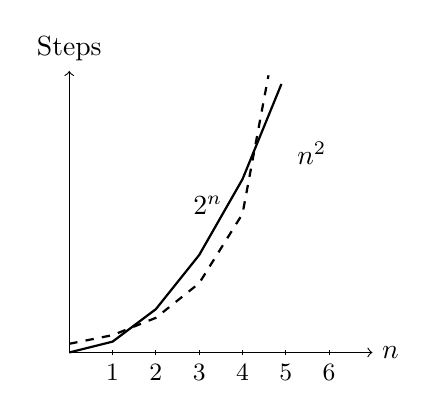
\begin{tikzpicture}[scale=0.55]
\draw[->] (0,0) -- (7,0) node[right] {$n$};
\draw[->] (0,0) -- (0,6.5) node[above] {Steps};
\draw[thick] (0,0) -- (1,0.25) -- (2,1) -- (3,2.25) -- (4,4) -- (4.9,6.2);
\node at (5.6,4.6) {$n^2$};
\draw[thick,dashed] (0,0.2) -- (1,0.4) -- (2,0.8) -- (3,1.6) -- (4,3.2) -- (4.6,6.4);
\node at (3.2,3.4) {$2^n$};
\foreach \x in {1,...,6} \draw (\x,0.05) -- (\x,-0.05) node[below] {\small \x};
\end{tikzpicture}
\end{center}

\begin{zhu}
This is only a schematic sketch. Both curves accelerate, but exponential growth soon leaves every polynomial far behind, though they may look similar at small $n$. That is the value of asymptotic thinking: examining the long-term trend.
\end{zhu}

The chasm is not just academic. Encryption used in shopping and logging in rests on easy verification and difficult inversion: multiplying large primes is easy, but splitting a hundreds-digit product is beyond even supercomputers working together. If someone proved P equals NP and produced a fast algorithm, modern cryptography's foundations would shake.

\section{Computers Return the Favour to Mathematics}

We have emphasised limitations: brute-force checks are not proofs; some problems cannot be computed, others take too long. Concluding that computers are useless to mathematics would be utterly wrong. The real picture is more interesting: they are transforming mathematics in at least three ways.

\subsection{Mass Computation as Part of Proof: The Four-Colour Theorem}

In 1852, someone asked whether four colours suffice for a map with differently coloured neighbours. This troubled mathematicians for over 120 years. In 1976, two mathematicians announced an unprecedented proof: reduce the problem to \textbf{over a thousand} basic configurations and check them all by computer. The theorem held, but over a thousand steps were performed by machine, beyond any person's hand-checking.

The mathematical world erupted: was this a proof? Could anyone trust what no human could independently check? Debate lasted years. The mainstream view now accepts exhaustive machine calculation as part of proof if the programme is carefully audited and its logic explicit. Later versions simplified and reverified the argument. Yet the theorem permanently changed proof's meaning: \textbf{reliability shifted from every capable person being able to recheck everything to every logical link being open to scrutiny, even if only a machine can execute one of them}.

\subsection{Machines as Proofreaders: Formal Proof}

A more radical approach avoids debating whether machine-assisted proofs count by writing the \textbf{entire} proof in a precise, machine-checkable language. This is formal proof. Assistants such as Lean and Coq require every inference to be unambiguous, then check the logic line by line. Humans supply ideas; machines find mistakes.

The work is painstaking but remarkably rewarding. A famous case is the Kepler conjecture: identical balls pack most densely in the familiar greengrocer's arrangement. Intuitively obvious, it was extraordinarily difficult to prove. In 1998, Hales announced a proof involving substantial computation. After years of checking, referees could only report ninety-nine per cent confidence; the remaining doubt concerned computations too extensive to check. Hales launched a project to formalise the whole proof. In 2014, machines certified every logical step, dispelling the doubt.

\begin{pandeng}
\textbf{Further Climbing}

Look for these keywords: \textbf{Turing machines}, the mathematical model of algorithms underpinning computer science; \textbf{P versus NP}, a million-dollar Millennium Prize Problem; \textbf{Hilbert's tenth problem}, undecidability of Diophantine solvability; \textbf{Lean}, a proof assistant helping mathematicians gradually machine-check modern mathematics; and \textbf{SAT solvers}, industrial-strength search engines for verifying chip logic.
\end{pandeng}

\subsection{Machines as Telescopes: Exploring Geometry, Number Theory, and Analysis}

The computer's most romantic role is telescope and microscope: helping humans \textbf{see} previously invisible mathematical worlds, while leaving proof to people.

In \textbf{geometry}, computers plotted iteration and revealed a whole new world. The Mandelbrot set arises by repeatedly applying $z \mapsto z^2 + c$ to complex numbers and colouring non-escaping points black. Its boundary contains layers of fractal detail, with fresh patterns at every enlargement, endlessly. Before computers, nobody knew such a simple formula concealed such intricate geometry. Fractal geometry now describes coastlines, clouds, and blood vessels.

In \textbf{number theory}, computers are enormous sieves. The largest known prime is a Mersenne prime with over twenty million digits, found by worldwide volunteers networking idle computers through GIMPS. Computers also verify Goldbach's conjecture---every even number greater than $2$ is a sum of two primes---over enormous ranges and record fine patterns in prime distribution. Such data inspire conjectures and sometimes supply ammunition to overturn them.

In \textbf{analysis}, numerical experiments often reveal patterns before theory. A legendary example is the BBP formula for $\pi$: computer searches first uncovered a formula extracting any chosen hexadecimal digit of $\pi$ directly, with rigorous proof following later. The machine sees the pattern first; humans then understand why. This reversed order is the classic workflow of experimental science.

\begin{toolbox}
\textbf{This Chapter's Mathematical Toolbox}

\begin{itemize}
\item \textbf{Finite verification $\neq$ proof}: However numerous, finite checks supply evidence. One counterexample refutes a conjecture; a proof must cover infinitely many cases.
\item \textbf{Algorithms}: Finite, explicit, necessarily terminating instructions, giving precision to mechanical solvability.
\item \textbf{Halting problem}: Some questions are algorithmically undecidable \textbf{in principle}; self-reference and contradiction expose such barriers.
\item \textbf{Computational complexity}: Among algorithmic problems, distinguish fast from slow. Polynomial growth is manageable, exponential growth monstrous; P versus NP remains a great mystery.
\item \textbf{Human--machine teamwork}: Machines perform massive calculations, rigorous checks, and visual exploration; humans ask questions, invent concepts, and supply insight-dependent reasoning.
\end{itemize}
\end{toolbox}

\section{A Paper Computer Lab: Hands-On Experiments}

\begin{shiyan}
\textbf{Experiment 1: Run $3n+1$ by hand.}

Start with $27$ and apply the rule on paper: divide evens by $2$, multiply odds by $3$ and add $1$. Patiently count the steps to $1$, around a hundred, and record the largest value. This small $27$ rises as high as $9232$ before falling. Try $31$ or $97$ too. Feel why verification is not effortless: trajectories rise and fall unpredictably, yet \textbf{so far} every tested one lands safely.

\textbf{Experiment 2: Feel binary search with books.}

Arrange $16$ books by spine height or page number. Ask a classmate to choose one mentally. You may ask only whether it is a selected book or lies to its left or right. Always start in the middle and record the maximum questions needed. Then search from the first book sequentially and record the worst case. For $16$ books, binary search needs at most $4$ checks, sequential search $16$. Repeat with $32$: binary search adds just $1$ check, while sequential search doubles. Handle logarithmic and linear growth yourself and you will not forget the difference.

\textbf{Experiment 3: Sketch the lying programme.}

Work only on paper. Suppose your deskmate claims a universal programme $H$ detects whether any programme loops forever. Following the proof, describe the contrary programme $D$ and ask whether $D$ halts on $D$. Whatever the answer, identify the contradiction. This game gives tangible understanding of contradiction and self-reference.
\end{shiyan}

\section*{Questions to Think About}

\textbf{Observation}

1. Evaluate $n^2 - n + 41$ for $n=1,2,\dots,8$, check primality, then calculate directly at $n=41$. Hint: at $n=41$, the first two terms $41^2-41$ share a factor $41$, so the whole expression has factor $41$.

2. In the $3n+1$ process, what must the final few values of any trajectory reaching $1$ be? Hint: which number becomes $1$ after division by $2$? Then work backwards once more.

\textbf{Proof}

3. Imitate the halting proof to show no algorithm $G$ can accept any programme $P$ such that $G$ always decides correctly whether $P$ prints the two-character Chinese greeting ni hao, meaning hello. Hint: assume $G$ exists and build a programme that asks $G$ whether it will print hello, refuses if told yes, and prints it if told no; then have it judge itself.

4. Prove that binary search finds any one of $n$ ordered books within at most $\lceil \log_2 n \rceil + 1$ checks. Hint: each check at least halves the search range. How many halvings reduce $n$ to $1$?

\textbf{Challenge}

5. Someone announces a proof that P equals NP and a polynomial-time Sudoku algorithm. Assuming this is correct, name three aspects of everyday life that would change radically, with reasons. Hint: recall cryptography, then think further: is checking a mathematical proof difficult? If easily verified things are easily found, what would automatic theorem proving mean?

6. The $3n+1$ conjecture is unproved. Someone suggests that, since halting is undecidable, perhaps the $3n+1$ conjecture is inherently undecidable too. Which parts of that reasoning are defensible, and which confuse concepts? Hint: no universal algorithm deciding \textbf{all} programmes differs from \textbf{one} particular statement being unprovable. Nonetheless, mathematicians have constructed specific number-theoretic problems equivalent to halting.

\section*{The Door to the Next Chapter}

We have seen a strange picture. Computers are humanity's most powerful calculating tools, capable of checking thirty quadrillion numbers in a blink, auditing proofs longer than a lifetime's checking, and drawing unimaginable fractals. Yet insurmountable walls remain: some problems have no algorithm, some algorithms take too long, and a hundred million verifications still do not mean universally true.

Machines' power and boundaries reflect mathematics' own. Godel makes incompleteness unavoidable for sufficiently strong axiomatic systems; Turing makes undecidability an unavoidable reef for computation. Unsolved questions such as P versus NP remind us that much beneath our proud mathematical building remains unexplored.

What are those foundations? How did nineteenth-century mathematicians shore up limits, infinity, and continuity, concepts that make school mathematics feel less secure? How do deep theorems, from the fundamental theorem of calculus to Galois theory, stitch apparently unrelated branches into one map? Next we stand at mathematics' edge and look back at the whole: where are its boundaries, and where does its map lead?
